\documentclass[12pt]{article}
\usepackage{array}
\usepackage{amsmath}
\usepackage{mathtools}
\usepackage{gensymb}
\usepackage{graphicx}
\usepackage{float}
\usepackage{caption}

\allowdisplaybreaks

\begin{document}
    \title{Moment of Inertia of a Steel Rod}
    \author{Ryan Coyne and Patrick Browning}
    \maketitle
    \section{Abstract}
        The moment of inertial of a metal bar was measured using weights and a rotational motion sensor. The moment of inertia was approximated to be 0\(.0094~\mathrm{kg\cdot m}^2\) based on the volume and density of the rod and was measured to be \((0.0116 \pm 0.00014)~\mathrm{kg\cdot m^2}\). The mechanical energy of the system of the rod and the weights was also analyzed. Mechanical energy graphed versus time was mostly consistent over time.
    \section{Introduction}
        An object's moment of inertia can be approximated using it's mass and an equation based on it's shape. For a cylindrical rod rotating on an axis that is perpendicular to it's length and which passes through it's center of mass, the equation that models it's moment of inertia is
        \begin{equation*}
            I = \frac{1}{12}mL^2
        \end{equation*}
        where \(I\) is the moment of inertia, \(m\) is the total mass of the rod and \(L\) is the full length of the rod. This is an approximation but it is possible to experimentally measure a more precise value for \(I\).
        
        The moment of inertia of an object determines how easily it's angular velocity can be changed. This change is done by torque on the system can be found using the equation \(\tau = I \alpha\) where \(\tau\) is the torque and \(\alpha\) is the angular acceleration. Using this equation along with Newton's second law of motion and the identity \(\alpha = \frac{a}{r}\) where \(a\) is the tangential acceleration of the rotating body and \(r\) is the radius of the rotating body. The equation
        \begin{equation*}
            \frac{1}{a} = \frac{I}{mgR^2}+\frac{1}{g}
        \end{equation*} 
        can be found from these. This equation shows that \(\frac{1}{a}\) is proportional to \(\frac{1}{m}\). If points are plotted with \(\frac{1}{a}\) as the y-axis and \(\frac{1}{m}\) as the x-axis then the slope of the line is \(S = \frac{I}{gR^2}\). Rearranging we find:
        \begin{equation*}
            I = SgR^2
        \end{equation*}

        The mechanical energy of the system should be conserved. There are small non-conservative forces on system, which are air resistance on the falling mass and the rotating rod, and friction between the bearings and the rotating axle, and friction on the rotational motion sensor. These non-conservative forces should decrease the total mechanical energy slightly but this decrease should be negligible.
    \section{Procedure}
        A horizontal metal bar and pulley were mounted on a vertical with the axle through their centers of mass. The axle was put on bearings in a metal frame so that it can rotate freely. The frame was placed on a table and a rotational motion sensor was mounted above the edge of the table. A string was attached to and wrapped around the pulley. The string was then draped over the rotational motion sensor. The metal frame was lined up so that the string was parallel to the directions of rotation of the pulley and the sensor.

        The bar was held still so that it would not rotate and a one hundred gram weight was hung from the end of the string. The sensor was turned on and started recording at which point the metal rod was released to spin. When the string had fully unwound from the pulley, the recording was stopped. This was repeated six more times with an additional twenty grams added to the hanging weight for each trial.
        \begin{figure}
            \centering
            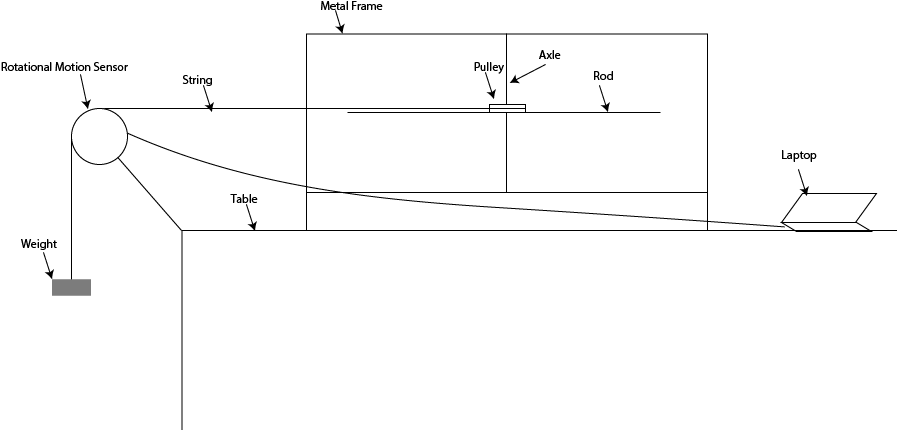
\includegraphics[width=0.75\linewidth]{Setup.png}
            \caption{Experimental Setup}
        \end{figure}
    \section{Data}
        \begin{center}
            \begin{tabular}{c|c}
                Trial & \(D\) (m)\\
                \hline
                1 & 0.0590\\
                2 & 0.0596\\
                3 & 0.0598\\
                4 & 0.0594\\
                \hline
                \(\overline{x}\) & 0.05945\\
                \(\sigma_x\) & 0.00034
            \end{tabular}\\
            Table 1. Pulley Diameter\\[12pt]
            \begin{tabular}{c|cc}
                Trial & \(m\) (kg) & \(a\) (m/s\(^2\))\\
                \hline
                1 & 0.10 & 0.0779\\
                2 & 0.12 & 0.0944\\
                3 & 0.14 & 0.1113\\
                4 & 0.16 & 0.1296\\
                5 & 0.18 & 0.1452\\
                6 & 0.20 & 0.1644\\
                7 & 0.22 & 0.1798\\
            \end{tabular}\\
            Table 2. Dependance of Acceleration on Hanging Mass\\[12pt]
            \(I\) was estimated to be 0.0116 \(\mathrm{kgs^2/m}\) from \(L_{\mathrm{metal}} = 0.6037\) m and \(D_{\mathrm{metal}} = 0.00927\) m.\\
            The mass \(m\) used for the conservation of energy analysis was \(0.12\) kg.
        \end{center}
        \begin{figure}[H]
            \centering
            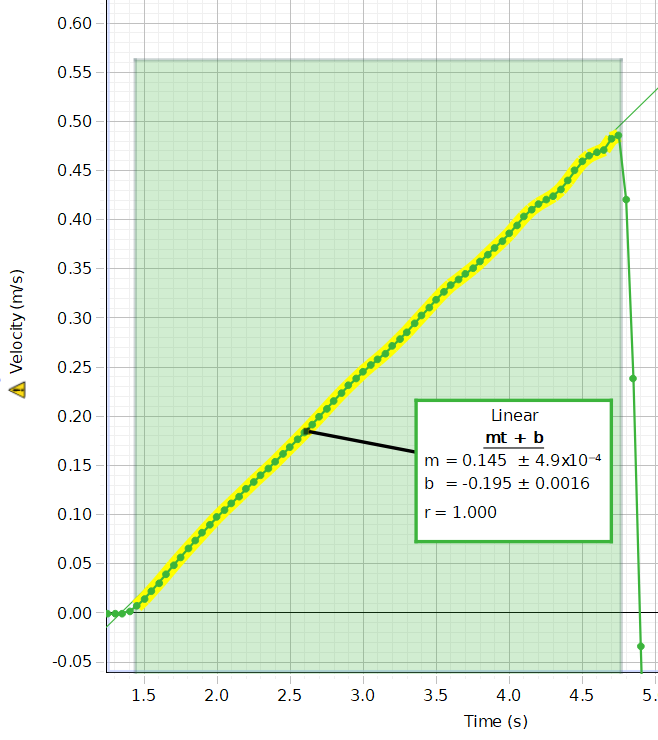
\includegraphics[width=0.75\linewidth]{acelleration fit.png}
            \caption{Sample Plot of Velocity vs Time with Fit to Determine Acceleration}
        \end{figure}
        \begin{figure}[H]
            \centering
            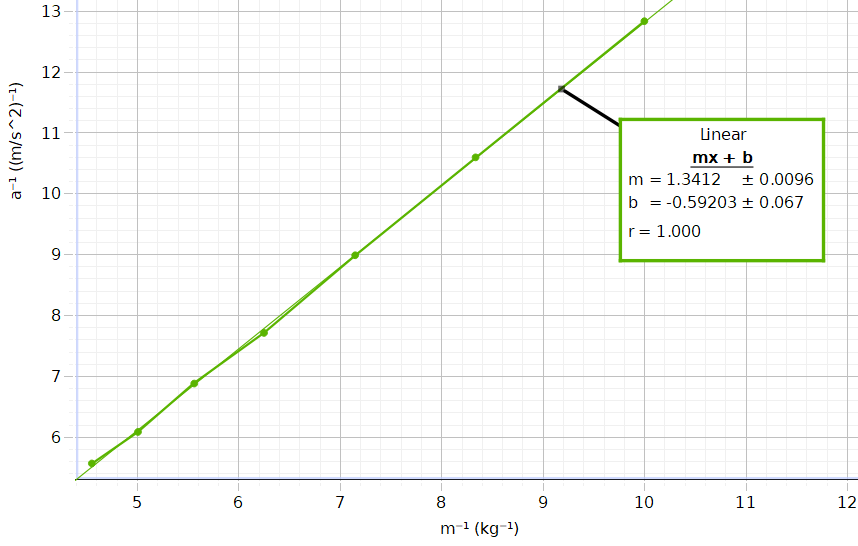
\includegraphics[width=0.75\linewidth]{a vs m.png}
            \caption{Plot of 1/\(a\) vs 1/\(m\) with Fit}
        \end{figure}
        \begin{figure}[H]
            \centering
            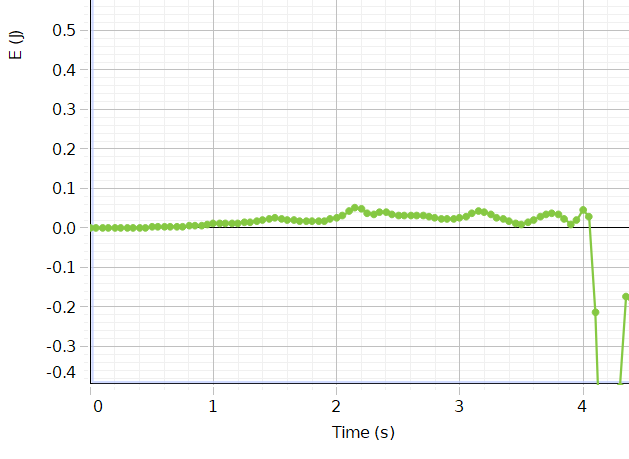
\includegraphics[width=0.75\linewidth]{mechE.png}
            \caption{Plot of Mechanical Energy vs Time}
        \end{figure}
        \pagebreak
    \section{Calculations}
        \begin{alignat*}{3}
            (1)~
            &&mg-T &= ma\\
            &&mg &= ma + T\\
            &&\tau &= I\frac{a}{R}\\
            &&TR &= I\frac{a}{R}\\
            &&T &= I\frac{a}{R^2}\\
            &&mg&=ma+I\frac{a}{R^2}\\
            &&mg&=a\left(m+\frac{I}{R^2}\right)\\
            &&a&=\frac{mg}{m+\frac{I}{R^2}}\\
            &&\frac{1}{a} &= \frac{m+\frac{I}{R^2}}{mg}\\
            &&\frac{1}{a} &= \frac{I}{mgR^2}+\frac{1}{g}\\
            (2)~
            &&I &\approx\frac{1}{12}ML^2\\
            &&M &= \pi \rho L_{\mathrm{metal}} \frac{D_{\mathrm{metal}}^2}{4}\\
            &&& = \pi \cdot 8000~\mathrm{kg/m}^2 \cdot \frac{(0.00927~\mathrm{m})^2}{4}\\
            &&& = 0.326~\mathrm{kg}\\
            &&I &\approx \frac{1}{12}0.326 ~\mathrm{kg} \cdot (0.6037~\mathrm{m})^2\\
            &&&\approx 0.00990~\mathrm{kg\cdot m}^2\\
            (3)~
            &&I &= SgR^2\\
            &&& = 1.3412~\mathrm{kg\cdot s^2 /m} \cdot 9.8~\mathrm{m/s^2} \cdot (0.0297~\mathrm{m})^2\\
            &&& = 0.0116 ~\mathrm{kg\cdot m^2}\\
            (4)~
            &&I_S &= (1.3412 + 0.0096)~\mathrm{kg\cdot s^2 /m} \cdot 9.8~\mathrm{m/s^2} \cdot (0.0297~\mathrm{m})^2\\
            &&&= 0.0117 ~\mathrm{kg\cdot m^2}\\
            &&I_R &= 1.3412~\mathrm{kg\cdot s^2 /m} \cdot 9.8~\mathrm{m/s^2} \cdot ((0.0297+0.00017)~\mathrm{m})^2\\
            &&&= 0.0117~\mathrm{kg\cdot m^2}\\
            &&\sigma_I &= \sqrt{((0.0117-0.0116)~\mathrm{kg\cdot m^2})^2+((0.0117-0.0116)~\mathrm{kg\cdot m^2})^2}\\
            &&& = 0.00014~\mathrm{kg\cdot m^2}
        \end{alignat*}
    \section{Conclusion}
        The approximated moment of inertia for the steel rod is within two standard deviations of the measured moment of inertia. This indicates that it is a good approximation for the moment of inertia. Systematic error may have arisen from the alignment of the pulleys and string because they were aligned by sight and not by using any more precise method. The graph of mechanical energy is mostly flat with some wobbling that is likely a result of random error.
\end{document}